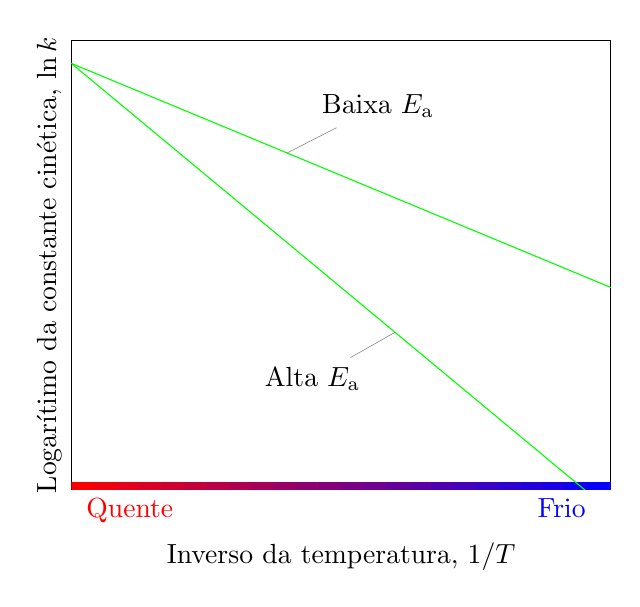
\begin{tikzpicture}
    \begin{axis}
        [
            xlabel = {Inverso da temperatura, $1/T$},
            ylabel = {Logarítimo da constante cinética, $\ln k$},
            xmin = 0, xmax = 5,
            ymin = 0, ymax = 5,
            domain = 0:5,
            ytick = \empty,
            xtick = { 0.5, 4.5 },
            xticklabels = 
                { 
                    { \color{red} Quente }, 
                    { \color{blue} Frio }, 
                },
            xtick style = { draw=none },
        ]
    \addplot 
        [
            mesh,
            colormap={}{
                color(0cm)=(red);
                color(1cm)=(blue);
            },
            line width = 1.2ex,
            point meta = x
        ]
        { 0 };
    \addplot 
        [
            green
            % mesh,
            % colormap={}{
            %     color(0cm)=(red);
            %     color(1cm)=(blue);
            % },
            % ultra thick,
            % point meta = x
        ]
        { 4.75 - x };
    \addplot 
        [
            green
            % mesh,
            % colormap={}{
            %     color(0cm)=(red);
            %     color(1cm)=(blue);
            % },
            % ultra thick,
            % point meta = x
        ]
        { 4.75 - 0.5*x };
    \node[coordinate, pin=above right:{Baixa $E_\mathrm{a}$}] 
        at (axis cs:2,3.75)   {};
    \node[coordinate, pin=below left:{Alta $E_\mathrm{a}$}] 
        at (axis cs:3,1.75)   {};
    \end{axis}
\end{tikzpicture}
